\chapter{Anexo}

    \section{Problemas y Ejercicios}
        En esta sección se aborda la solución de los problemas solicitados durante las clases previas a la práctica. 

        \subsection{Ejercicio 1}
            \textit{Descripción}: Probar mediante sustitución hacia atrás que \(T(n) \in \Theta (n\log(n) ) \)
            
                \begin{figure}[htp!]
                    \centering
                    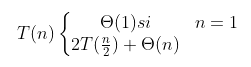
\includegraphics[width=0.3 \textwidth]{Images/eee.png}
                    \label{fig:1}
                \end{figure}
            Resolviendo se tiene \(n = 2^{k}\) entonces \(T(2^{k}) = 2T(2^{k-1}+c2^{k})\)
                \begin{gather*}
                    T(2^{k})=2T(2^{k-1}+c2^{k}\\
                    T(2^{k})=2[2T(2^{k-2}+c2^{k-1}] + c2^{k}\\
                    T(2^{k})=2^{2}T(2^{k-2}) + 2c2^{k}\\
                    T(2^{k})=2^{2}[2T(2^{2k-3}) + c2^{k-2}] + 2c2^{k}\\
                    T(2^{k})=2^{3}T(2^{k-3}) + c2^{k} + 2c2^{k}\\
                    T(2^{k})=2^{3}T(2^{k-3}) + 3c2^{k}\\
                    T(i)=2^{i}T(2^{k-i}) + ic2^{k}\\
                    % \therefore  T(n)\in O(n)
                \end{gather*}
            
            Teniendo que \(k-1 = 0\) y \(k = 1\)
                \begin{gather*}
                    = 2^{k}T(2^{0}+k(2^{k})\\
                    = 2^{k}c+kc2^{k}\\
                    = (c + kc)(2^{k})\\
                    = (c + c\log_{2}n)n\\
                    \therefore T(n)\in \theta (n\log{n})
                    % \therefore  T(n)\in O(n)
                \end{gather*}

        \newpage
        \subsection{Ejercicio 2}
            \textit{Descripción}: Utilizando decremento por uno, pruebe que \(T(n) \in O(n^{2}\)

            Teniendo que \(T(n) = T(n-1) + c(n+1)\) resolvemos:
                \begin{gather*}
                    = T(0)+\sum_{j=1}^{n}f(j)\\
                    = T(0)+\sum_{j=1}^{n}c(j+1)\\
                    = T(0)+\sum_{j=1}^{n}c(2+3+4+... + (n+1)) = c(n+1)(n+2)\\
                    = cn^{2} + c3n + 2c - 2c \\
                    = \frac{c(n^{2} + 3n)^{2}}{2}\\
                    \therefore T(n)\in O (n^{2})
                    % \therefore  T(n)\in O(n)
                \end{gather*}
                
        \subsection{Ejercicio 3}
            \textit{Descripción}: Utilizando el teorema maestro, pruebe que \(T(n) \in A = \Omega(n\log{n})\)
            \
            \newline
            Teniendo que \(T(n) = 2T(\frac{n}{2}) + \theta(n)\) es \(= T(n) = 2T(\frac{n}{2}) + Cn\\\)

            Resolviendo se tiene que \(a=2, b=2, f(n) = cn\)
                \begin{gather*}
                    cn = \theta(n^{log_{2}2})\\
                    \theta(n^{log_{2}2}\log{n}) = \theta(n\log{n}) \\
                    \therefore T(n)\in \theta(n\log{n})
                    % \therefore  T(n)\in O(n)
                \end{gather*}

        \subsection{Ejercicio 4}
            \textit{Descripción}: Mediante Teorema Maestro, pruebe que \(T(n) \in \theta(n^{2})\)
            \newline
            Con \(T(n) = 4T(\frac{n}{2}) + \theta(n)\) se tiene \(a=4, b=2, f(n) = cn\)
            \newline
            Por el caso (III) del Teorema Maestro se obtiene: 
                \begin{gather*}
                    \theta(n^{log_{2}4})\\
                    \therefore T(n)\in \theta(n^{2})
                    % \therefore  T(n)\in O(n)
                \end{gather*}
        \newpage
        \subsection{Ejercicio 5}
            \textit{Descripción}: Mediante Teorema Maestro, pruebe que \(T(n) \in \theta(n^{\log{3}})\)
            \newline
            Con \(T(n) = 3T(\frac{n}{2}) + \theta(n)\) se tiene \(a=3, b=2, f(n) = cn\)
            \newline
            Por el caso (III) del Teorema Maestro se obtiene: 
                \begin{gather*}
                    \theta(n^{log_{2}3})\\
                    \therefore T(n)\in \theta(n^{log_{2}3})
                    % \therefore  T(n)\in O(n)
                \end{gather*}
                
        \subsection{Ejercicio 6}
            \textit{Descripción}: Mediante Teorema Maestro, pruebe que \(T(n) \in \theta(n\log{n})\)
            \newline
            Con \(T(n) = 2T(\frac{n}{2}) + \theta(n)\) se tiene \(a=2, b=2, f(n) = cn\)
            \newline
            Por el caso (II) del Teorema Maestro se obtiene: 
                \begin{gather*}
                    \theta(n^{log_{2}3})\\
                    \therefore T(n)\in \theta(n\log{n})
                    % \therefore  T(n)\in O(n)
                \end{gather*}